% chapters/04_firmware_implementation.tex - Chapter 4: Firmware Implementation
% =============================================================================

\chapter{Embedded Firmware Design}
\label{chap:firmware-implementation}

The firmware running on the ESP32-S3 forms the foundation of the Rescue Rover system \cite{lee2017embedded}. This chapter documents the design decisions, implementation details, and technical challenges encountered while developing the embedded software layer. The firmware handles camera streaming, motor control, wireless communication, and safety mechanisms, all running concurrently on the dual core processor.

% --------------------------------------------------------
\section{Firmware Architecture Overview}
\label{sec:firmware-overview}

The ESP32-S3 firmware follows a modular architecture where each hardware subsystem is encapsulated in its own compilation unit. This separation allows independent development and testing of each component before integration. The project contains five primary modules, each with a specific responsibility in the system.

% FIGURE PLACEHOLDER
\begin{figure}[H]
    \centering
    \includegraphics[width=\textwidth]{figures/software/firmware_architecture.png}
    \caption{Firmware module architecture showing the main sketch and its dependencies. The main loop coordinates all subsystems while individual modules manage their respective hardware interfaces.}
    \label{fig:firmware-architecture}
\end{figure}

\subsection{Module Responsibilities}

The \texttt{RescueRobot.ino} file serves as the main entry point. It initializes all hardware subsystems in a specific order and runs the main control loop at approximately 60Hz. The loop coordinates sensor readings, command processing, safety checks, and telemetry transmission. Total line count for this file is 265 lines.

The \texttt{CameraModule} handles all camera operations. This includes initialization of the OV2640 sensor, configuration of frame buffers in PSRAM, and streaming via either HTTP or UDP protocols. The module provides two streaming modes because we discovered during testing that HTTP introduces 80ms additional latency compared to UDP on the same network. Total implementation spans 222 lines across the header and source files.

The \texttt{MotorDriver} module controls the L298N H bridge through GPIO pins \cite{stmicro2000l298,mishra2018implementation}. Movement primitives include forward, backward, left turn, right turn, and emergency stop. The implementation uses \textbf{PWM (Pulse Width Modulation)} to enable variable speed control, with a speed parameter from 0\% to 100\% mapped to PWM duty cycles 0-255 \cite{siegwart2011robotics}. This module spans 92 lines.

The \texttt{ConnectionModule} manages ESP NOW bidirectional communication with the gateway. It receives joystick commands, stores them for processing by the main loop, and transmits telemetry at 2Hz. The critical design decision here is that the receive callback does not directly actuate motors. Instead it stores the command and lets the main loop apply safety checks first. This prevents race conditions between sensor readings and motor commands.

% FIGURE PLACEHOLDER
\begin{figure}[H]
    \centering
    \includegraphics[width=\textwidth]{figures/software/module_dependencies.png}
    \caption{Compilation dependencies between firmware modules. The main sketch includes all headers while modules only include what they need.}
    \label{fig:module-dependencies}
\end{figure}

\subsection{Memory Layout}

The ESP32-S3 provides multiple memory regions with different characteristics. Understanding these regions is essential for camera buffer allocation and overall system stability.

\begin{table}[h!]
    \centering
    \caption{ESP32-S3 memory regions and their usage in the firmware}
    \label{tab:memory-regions}
    \begin{tabular}{llp{6cm}}
        \toprule
        \textbf{Region} & \textbf{Size} & \textbf{Usage in Firmware} \\
        \midrule
        Internal SRAM    & 512 KB & Stack, heap, global variables, WiFi buffers \\
        PSRAM (External) & 8 MB   & Camera frame buffers (2 x 320x240), JPEG output buffer \\
        Flash            & 16 MB  & Program code, string constants, WiFi credentials \\
        \bottomrule
    \end{tabular}
\end{table}

Camera frame buffers consume the majority of PSRAM. Each QVGA frame requires 320 x 240 x 2 = 153.6 KB in YUV format. We allocate two buffers for double buffering, allowing one to be transmitted while the other captures the next frame. The JPEG compressed output typically ranges from 5 KB to 15 KB depending on scene complexity.

% FIGURE PLACEHOLDER
\begin{figure}[h!]
    \centering
    \includegraphics[width=0.7\textwidth]{figures/hardware/esp32s3_memory_map.png}
    \caption{Memory allocation for the Rescue Rover firmware showing how camera buffers dominate PSRAM usage.}
    \label{fig:memory-map}
\end{figure}


% --------------------------------------------------------
\section{Camera Module Implementation}
\label{sec:camera-module-impl}

The camera module presented the most significant technical challenges during development. The OV2640 sensor requires precise timing, correct voltage levels, and specific initialization sequences. Several iterations were needed before achieving stable operation.

\subsection{Hardware Configuration}

The OV2640 connects to the ESP32-S3 through a DVP (Digital Video Port) interface. This parallel interface uses 8 data lines (D0-D7), synchronization signals (VSYNC, HREF, PCLK), and an I2C bus for register configuration.

\begin{figure}[h!]
    \centering
    % Define color BEFORE starting the tikzpicture environment
    \definecolor{gold}{HTML}{FFD700}

    \begin{tikzpicture}[
        node distance=2cm,
        font=\sffamily\footnotesize,
        thick,
        % Component Styles
        board/.style={draw=black!80, fill=white, rounded corners=4pt, drop shadow},
        esp32/.style={board, fill=blue!10, minimum width=4cm, minimum height=8cm},
        breakout/.style={board, fill=green!10, minimum width=2.5cm, minimum height=7cm},
        camera/.style={board, fill=black!80, minimum width=2.5cm, minimum height=2.5cm},
        % Pin Styles
        pinlabel/.style={font=\sffamily\scriptsize, align=right},
        gpiolabel/.style={font=\sffamily\scriptsize, align=left},
        % Usage of 'gold' is now valid because it was defined above
        headerpin/.style={circle, fill=gold, inner sep=1.5pt, draw=black!50},
        % Wire Styles
        wire/.style={line width=1.2pt, rounded corners=5pt},
        pwr/.style={wire, red},
        gnd/.style={wire, black},
        i2c/.style={wire, orange!80!black},
        clock/.style={wire, green!60!black},
        data/.style={wire, blue!70!black},
        nc/.style={wire, gray, dashed}
    ]

    % --- 1. ESP32-S3 Board (Right Side) ---
    \node[esp32] (esp) at (8,0) {};
    \node[above=0.2cm, font=\bfseries] at (esp.north) {ESP32-S3 Dev Board};

    % Define ESP32 Pin coordinates and labels
    % Left side headers
    \foreach \y/\lab in {3.5/3V3, 3.0/GND, 2.0/IO10, 1.5/IO13, 0.5/IO15, 0/IO17, -0.5/IO18, -1.0/IO16, -1.5/IO14, -2.0/IO12, -2.5/IO11} {
        \node[headerpin] (esp_l_\lab) at ($(esp.west) + (0.2, \y)$) {};
        \node[gpiolabel, right=0.1cm of esp_l_\lab] {\lab};
    }
    % Right side headers
    \foreach \y/\lab in {2.5/IO40, 2.0/IO39, 1.0/IO38, 0.5/IO47, -3.0/IO48} {
        \node[headerpin] (esp_r_\lab) at ($(esp.east) + (-0.2, \y)$) {};
        \node[gpiolabel, left=0.1cm of esp_r_\lab] {\lab};
    }

    % --- 2. FPC Breakout Board (Middle) ---
    \node[breakout] (brk) at (0,0) {};
    \node[above=0.2cm, font=\bfseries] at (brk.north) {FPC Breakout};

    % Define Breakout Pin coordinates and labels
    \foreach \y/\lab/\type in {
        3.5/3V3/pwr, 3.0/GND/gnd, 
        2.5/SIOD/i2c, 2.0/SIOC/i2c,
        1.5/XCLK/clock, 1.0/PCLK/clock, 0.5/VSYNC/clock, 0.0/HREF/clock,
        -0.5/D0/data, -1.0/D1/data, -1.5/D2/data, -2.0/D3/data, 
        -2.5/D4/data, -3.0/D5/data, -3.5/D6/data, -4.0/D7/data,
        -4.5/PWDN/nc, -5.0/RESET/nc
    } {
        \node[headerpin] (brk_\lab) at ($(brk.east) + (-0.2, \y)$) {};
        \node[pinlabel, left=0.1cm of brk_\lab] {\lab};
    }

    % --- 3. Camera Module (Left Side) ---
    \node[camera, left=2cm of brk] (cam) {};
    \node[above=0.2cm, font=\bfseries, align=center] at (cam.north) {OV2640\\Module};
    % Lens representation
    \draw[fill=black, draw=gray, thick] (cam.center) circle (0.8cm);
    \draw[fill=blue!10!black, draw=black] (cam.center) circle (0.3cm);

    % --- Ribbon Cable Connection ---
    \draw[line width=10pt, gray!40, shorten >=-2pt, shorten <=-2pt] (cam.east) -- (brk.west);
    \node[font=\tiny\sffamily, color=black!60, rotate=0, align=center, fill=white, opacity=0.8] at ($(cam.east)!0.5!(brk.west)$) {24-Pin FPC\\Ribbon Cable};


    % --- 4. Wiring Connections ---

    % Power
    \draw[pwr] (brk_3V3) -- ++(1,0) |- (esp_l_3V3);
    \draw[gnd] (brk_GND) -- ++(0.8,0) |- (esp_l_GND);

    % I2C (Control)
    \draw[i2c] (brk_SIOD) -- ++(1.5,0) |- (esp_r_IO40);
    \draw[i2c] (brk_SIOC) -- ++(1.7,0) |- (esp_r_IO39);

    % Clocks & Sync
    \draw[clock] (brk_XCLK) -- ++(1.2,0) |- (esp_l_IO10);
    \draw[clock] (brk_PCLK) -- ++(1.4,0) |- (esp_l_IO13);
    \draw[clock] (brk_VSYNC) -- ++(1.9,0) |- (esp_r_IO38);
    \draw[clock] (brk_HREF) -- ++(2.1,0) |- (esp_r_IO47);

    % Data Bus (D0-D7 mapping to Y2-Y9)
    \draw[data] (brk_D0) -- ++(0.5,0) |- (esp_l_IO15);
    \draw[data] (brk_D1) -- ++(0.7,0) |- (esp_l_IO17);
    \draw[data] (brk_D2) -- ++(0.9,0) |- (esp_l_IO18);
    \draw[data] (brk_D3) -- ++(1.1,0) |- (esp_l_IO16);
    \draw[data] (brk_D4) -- ++(1.3,0) |- (esp_l_IO14);
    \draw[data] (brk_D5) -- ++(1.5,0) |- (esp_l_IO12);
    \draw[data] (brk_D6) -- ++(1.7,0) |- (esp_l_IO11);
    \draw[data] (brk_D7) -- ++(2.3,0) |- (esp_r_IO48);

    % Unused (NC) indicating software control or unconnected
    \draw[nc, ->] (brk_PWDN) -- ++(1,0) node[right, font=\tiny] {NC};
    \draw[nc, ->] (brk_RESET) -- ++(1,0) node[right, font=\tiny] {NC (SW Control)};

    % Legend
    \matrix [draw, fill=white, below right=0.5cm and 0cm of brk.south west, anchor=north west, nodes={font=\scriptsize, align=left}] {
        \draw[pwr, line width=2pt] (0,0) -- (0.5,0); & \node{Power (3.3V)}; \\
        \draw[gnd, line width=2pt] (0,0) -- (0.5,0); & \node{Ground}; \\
        \draw[i2c, line width=2pt] (0,0) -- (0.5,0); & \node{I2C Control}; \\
        \draw[clock, line width=2pt] (0,0) -- (0.5,0); & \node{Clocks/Sync}; \\
        \draw[data, line width=2pt] (0,0) -- (0.5,0); & \node{Data Bus}; \\
    };

    \end{tikzpicture}
    \caption{Physical wiring diagram illustrating the connections between the OV2640 camera module (via FPC breakout) and the ESP32-S3 development board.}
    \label{fig:camera-wiring}
\end{figure}

The pin mapping was derived from the Freenove ESP32-S3 WROOM CAM board schematic. However, our custom wiring required adjustments to avoid conflicts with motor control pins. The final configuration uses GPIO 10 for XCLK, GPIO 40 and 39 for I2C, and GPIO 38 for VSYNC. Data pins span GPIO 11 through 18 and GPIO 48.

\begin{lstlisting}[language=C++, caption={Camera pin configuration from CameraPins.h}]
// ESP32-S3 Camera Pin Mapping (Freenove Compatible)
#define PWDN_GPIO_NUM     -1   // Not connected
#define RESET_GPIO_NUM    -1   // Using software reset
#define XCLK_GPIO_NUM     10   // Master clock output
#define SIOD_GPIO_NUM     40   // I2C SDA
#define SIOC_GPIO_NUM     39   // I2C SCL
#define Y9_GPIO_NUM       48   // Data bit 7
#define Y8_GPIO_NUM       11   // Data bit 6
#define Y7_GPIO_NUM       12   // Data bit 5
#define Y6_GPIO_NUM       14   // Data bit 4
#define Y5_GPIO_NUM       16   // Data bit 3
#define Y4_GPIO_NUM       18   // Data bit 2
#define Y3_GPIO_NUM       17   // Data bit 1
#define Y2_GPIO_NUM       15   // Data bit 0
#define VSYNC_GPIO_NUM    38   // Vertical sync
#define HREF_GPIO_NUM     47   // Horizontal reference
#define PCLK_GPIO_NUM     13   // Pixel clock
\end{lstlisting}

\subsection{Initialization Sequence}

Camera initialization follows a strict sequence. Any deviation results in cryptic error codes or complete failure to capture frames. We reduced the XCLK frequency from 20MHz to 10MHz after encountering intermittent initialization failures. The lower clock speed sacrifices theoretical maximum framerate but dramatically improves reliability.

\begin{algorithm}[H]
    \caption{Camera Initialization Sequence}
    \label{alg:camera-init-full}
    \begin{algorithmic}[1]
        \STATE Check for PSRAM availability
        \IF{PSRAM not found}
            \STATE Log warning: camera may fail without external memory
        \ENDIF
        \STATE Populate \texttt{camera\_config\_t} structure with pin numbers
        \STATE Set XCLK frequency to 10 MHz (conservative setting)
        \STATE Set frame size to QVGA (320 x 240 pixels)
        \STATE Set pixel format to JPEG with quality level 30
        \STATE Set frame buffer location to PSRAM
        \STATE Allocate 2 frame buffers for double buffering
        \STATE Set grab mode to CAMERA\_GRAB\_LATEST
        \STATE Call \func{esp\_camera\_init} with configuration
        \IF{initialization returns error}
            \STATE Log error code and halt
            \RETURN false
        \ENDIF
        \STATE Get sensor handle via \func{esp\_camera\_sensor\_get}
        \STATE Disable test pattern (colorbar) for real images
        \STATE Log success message with resolution
        \RETURN true
    \end{algorithmic}
\end{algorithm}

% FIGURE: CAMERA INITIALIZATION FLOWCHART
\begin{figure}[H]
    \centering
    % Define styles for flowchart symbols
    \tikzset{
        font=\sffamily\footnotesize,
        base/.style = {draw=black, thick, align=center, minimum height=0.8cm},
        startstop/.style = {base, rounded corners, fill=red!10, minimum width=2.5cm},
        process/.style = {base, rectangle, fill=blue!10, minimum width=3.5cm, text width=3cm},
        decision/.style = {base, diamond, fill=yellow!10, aspect=2, inner sep=0pt},
        io/.style = {base, trapezium, trapezium left angle=70, trapezium right angle=110, fill=green!10, minimum width=3cm},
        arrow/.style = {thick, ->, >=Latex}
    }

    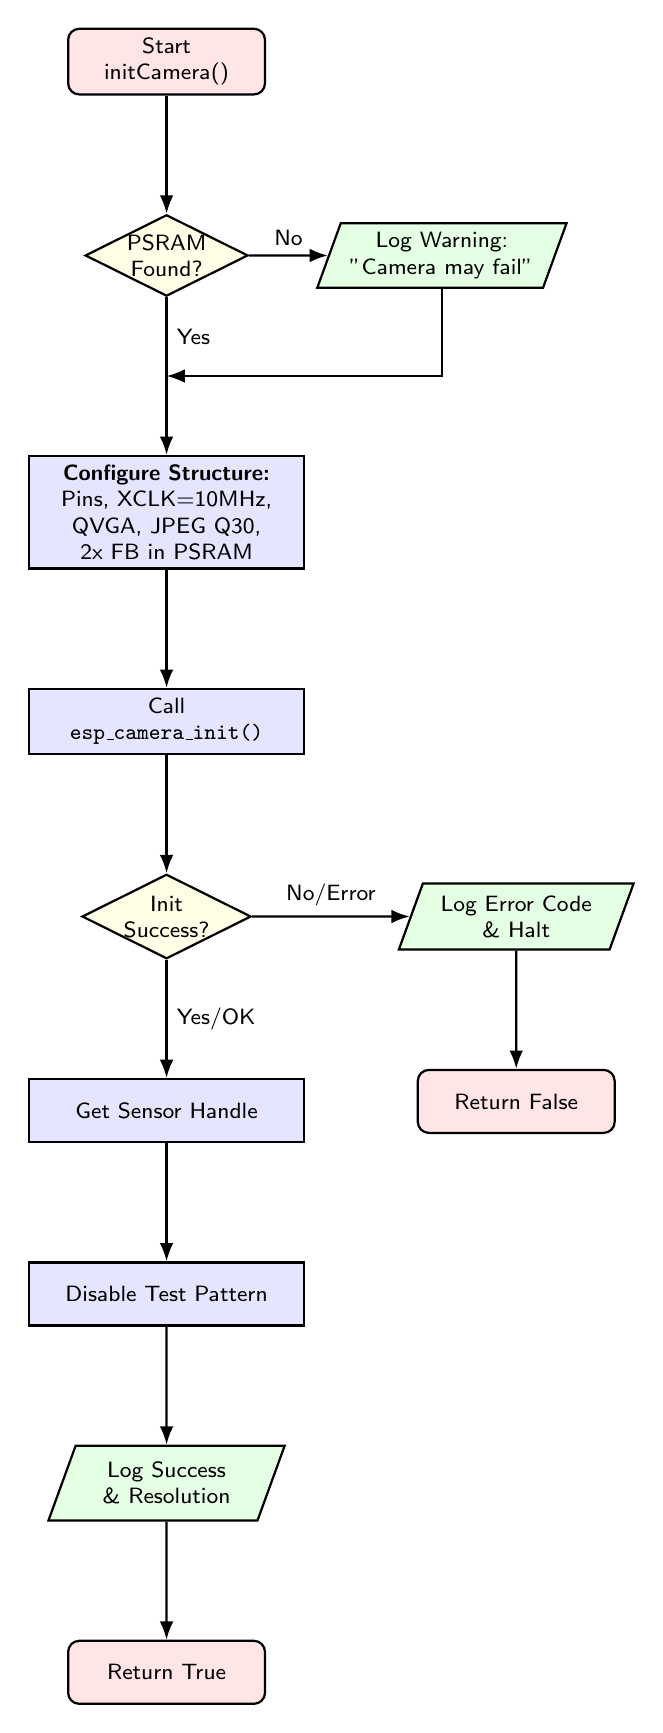
\begin{tikzpicture}[node distance=1.5cm and 1cm]
        % --- Nodes ---
        \node (start) [startstop] {Start\\initCamera()};
        
        \node (check_psram) [decision, below=of start] {PSRAM\\Found?};
        
        \node (log_warn) [io, right=of check_psram] {Log Warning:\\"Camera may fail"};

        % Combined configuration steps into one process block for clarity
        \node (config) [process, below=2cm of check_psram] {\textbf{Configure Structure:}\\Pins, XCLK=10MHz,\\QVGA, JPEG Q30,\\2x FB in PSRAM};
        
        \node (call_init) [process, below=of config] {Call\\\texttt{esp\_camera\_init()}};
        
        \node (check_success) [decision, below=of call_init] {Init\\Success?};
        
        % Failure Path (Right side)
        \node (log_err) [io, right=2cm of check_success] {Log Error Code\\\& Halt};
        \node (end_fail) [startstop, below=of log_err] {Return False};

        % Success Path (Straight down)
        \node (get_sensor) [process, below=1.5cm of check_success] {Get Sensor Handle};
        \node (disable_test) [process, below=of get_sensor] {Disable Test Pattern};
        \node (log_ok) [io, below=of disable_test] {Log Success\\\& Resolution};
        \node (end_ok) [startstop, below=of log_ok] {Return True};


        % --- Paths ---
        \draw [arrow] (start) -- (check_psram);
        
        % PSRAM Check paths
        \draw [arrow] (check_psram) -- node[above] {No} (log_warn);
        % Create a merge point for after the warning
        \coordinate (merge_psram) at ($(check_psram.south)!0.5!(config.north)$);
        \draw [arrow] (check_psram) -- node[right] {Yes} (merge_psram) -- (config);
        \draw [arrow] (log_warn) |- (merge_psram);
        
        % Main Flow
        \draw [arrow] (config) -- (call_init);
        \draw [arrow] (call_init) -- (check_success);
        
        % Init Success Check paths
        \draw [arrow] (check_success) -- node[above] {No/Error} (log_err);
        \draw [arrow] (log_err) -- (end_fail);
        
        \draw [arrow] (check_success) -- node[right] {Yes/OK} (get_sensor);
        
        % Final Success steps
        \draw [arrow] (get_sensor) -- (disable_test);
        \draw [arrow] (disable_test) -- (log_ok);
        \draw [arrow] (log_ok) -- (end_ok);

    \end{tikzpicture}
    \caption{Flowchart for camera initialization showing fail safe checks, critical configuration steps (including the reduced 10MHz XCLK), and error handling paths.}
    \label{fig:camera-init-flow}
\end{figure}

The JPEG quality parameter inversely correlates with file size. A quality value of 30 produces frames between 5KB and 12KB, suitable for UDP transmission within a single packet on local networks. Lower quality values (higher numbers in the ESP camera API) create smaller files but introduce visible compression artifacts.

\subsection{Streaming Modes}

The firmware supports two distinct streaming protocols. HTTP MJPEG provides browser compatibility and easy debugging. UDP streaming minimizes latency for the AI processing pipeline.

\subsubsection{HTTP MJPEG Streaming}

The HTTP mode creates a simple web server on port 80 with a single endpoint at \texttt{/stream}. When a client connects, the handler enters an infinite loop, capturing frames and sending them with multipart boundaries. This approach works with any web browser and requires no client side code.

\begin{lstlisting}[language=C++, caption={HTTP MJPEG stream handler implementation}]
static esp_err_t stream_handler(httpd_req_t *req) {
    camera_fb_t *fb = NULL;
    esp_err_t res = ESP_OK;
    char part_buf[64];
    
    // Set content type for MJPEG stream
    res = httpd_resp_set_type(req, 
        "multipart/x mixed replace;boundary=frame");
    if (res != ESP_OK) return res;
    
    while (true) {
        fb = esp_camera_fb_get();
        if (!fb) {
            Serial.println("Capture failed");
            res = ESP_FAIL;
        } else {
            // Build multipart header
            size_t hlen = snprintf(part_buf, 64,
                "\r\n--frame\r\n"
                "Content Type: image/jpeg\r\n"
                "Content Length: %u\r\n\r\n", fb->len);
            
            res = httpd_resp_send_chunk(req, part_buf, hlen);
            if (res == ESP_OK) {
                res = httpd_resp_send_chunk(req, 
                    (const char*)fb->buf, fb->len);
            }
            esp_camera_fb_return(fb);
        }
        if (res != ESP_OK) break;
    }
    return res;
}
\end{lstlisting}

% FIGURE PLACEHOLDER
\begin{figure}[H]
    \centering
    \includegraphics[width=\textwidth]{figures/software/http_stream_sequence.png}
    \caption{Sequence diagram for HTTP MJPEG streaming showing the continuous frame transmission loop.}
    \label{fig:http-sequence}
\end{figure}

\subsubsection{UDP Streaming (Experimental)}

UDP mode was initially designed to minimize latency by bypassing the HTTP overhead.

\begin{designbox}[UDP Buffer Overflow]
During integration testing, we observed that the ESP32-S3's network stack struggled to sustain high bandwidth UDP transmission at 30FPS. The internal buffers frequently overflowed, causing a \textbf{Watchdog Timer Reset} that crashed the system.

While UDP offered superior latency ($<$100ms), the instability was critical. We ultimately pivoted to TCP/HTTP for the final build. The TCP flow control mechanism prevents the application from overwhelming the network stack, ensuring system stability at the cost of slightly higher latency. Implementing a custom reliable UDP protocol was deemed out of scope for this iteration.
\end{designbox}

\begin{lstlisting}[language=C++, caption={UDP frame transmission function (Deprecated)}]
void streamFrameUDP() {
    // Check prerequisites
    if (!cameraReady || !udpMode || udpTargetIP == nullptr)
        return;
    
    camera_fb_t *fb = esp_camera_fb_get();
    if (!fb) return;
    
    // Chunking logic was attempted here but 
    // stack overflows persisted.
    udp.beginPacket(udpTargetIP, udpTargetPort);
    udp.write(fb->buf, fb->len);
    udp.endPacket();
    
    esp_camera_fb_return(fb);
}
\end{lstlisting}

% FIGURE PLACEHOLDER
\begin{figure}[h!]
    \centering
    \includegraphics[width=0.85\textwidth]{figures/charts/http_vs_udp_latency.png}
    \caption{Measured latency comparison between HTTP MJPEG and UDP streaming modes. UDP consistently shows 80ms lower latency.}
    \label{fig:latency-comparison}
\end{figure}

\begin{table}[h!]
    \centering
    \caption{Comparison of streaming modes}
    \label{tab:streaming-comparison}
    \begin{tabular}{lcc}
        \toprule
        \textbf{Characteristic} & \textbf{HTTP MJPEG} & \textbf{UDP Direct} \\
        \midrule
        End to end latency      & 180-220 ms    & 100-140 ms \\
        Browser compatible      & Yes           & No (requires custom receiver) \\
        Packet loss handling    & TCP retransmit & None (frames dropped) \\
        Setup complexity        & Low           & Medium \\
        Network overhead        & Higher        & Lower \\
        Recommended use         & Debugging     & Production \\
        \bottomrule
    \end{tabular}
\end{table}

% --------------------------------------------------------
\section{Motor Control Implementation}
\label{sec:motor-impl}

The motor control subsystem translates high level movement commands into GPIO signals for the L298N driver. The implementation uses \textbf{PWM speed modulation}, allowing both manual operators and AI modules to control the rover's velocity. A speed parameter (0-100\%) is mapped to a PWM duty cycle (0-255) using a linear conversion function.

\subsection{Differential Drive Model}

The rover uses a differential drive configuration with two independently controlled motors. This arrangement allows the robot to turn by varying the relative speeds of the left and right wheels. Mathematically, the relationship between wheel velocities and robot motion is expressed as:

\begin{equation}
    v_{robot} = \frac{v_R + v_L}{2}
    \label{eq:linear-vel}
\end{equation}

\begin{equation}
    \omega_{robot} = \frac{v_R - v_L}{W}
    \label{eq:angular-vel}
\end{equation}

where $v_{robot}$ is the linear velocity of the robot center, $\omega_{robot}$ is the angular velocity, $v_R$ and $v_L$ are the right and left wheel velocities respectively, and $W$ is the wheelbase width.

% FIGURE PLACEHOLDER
\begin{figure}[H]
    \centering
    \includegraphics[width=0.6\textwidth]{figures/hardware/differential_drive_kinematics.png}
    \caption{Differential drive kinematic model showing how independent wheel speeds create linear and angular motion.}
    \label{fig:diff-drive}
\end{figure}

\subsection{L298N Driver Interface}

The L298N accepts four digital inputs (IN1 through IN4) that control two H bridge circuits. Each motor connects to one H bridge. For direction control, one pin is set HIGH while the other is LOW. For speed control, the HIGH signal is replaced with a PWM waveform using \texttt{analogWrite()}.

\begin{lstlisting}[language=C++, caption={PWM based motor driver with speed control}]
#include "MotorDriver.h"
#include "PinConfig.h"

// Convert 0-100% speed to 0-255 PWM duty cycle
int speedToPWM(int speed) {
    return map(speed, 0, 100, 0, 255); 
}

void initMotors() {
    pinMode(PIN_LEFT_FWD, OUTPUT);
    pinMode(PIN_LEFT_BWD, OUTPUT);
    pinMode(PIN_RIGHT_FWD, OUTPUT);
    pinMode(PIN_RIGHT_BWD, OUTPUT);
    
    stopMoving();
    Serial.println("Motor Driver Ready (PWM Control Enabled)");
}

void goForward(int speed) {
    if (speed < 1 || speed > 100) return;
    int pwm = speedToPWM(speed);
    
    // Left motor forward
    analogWrite(PIN_LEFT_FWD, pwm);
    digitalWrite(PIN_LEFT_BWD, LOW);
    
    // Right motor forward
    analogWrite(PIN_RIGHT_FWD, pwm);
    digitalWrite(PIN_RIGHT_BWD, LOW);
}

void stopMoving() {
    digitalWrite(PIN_LEFT_FWD, LOW);
    digitalWrite(PIN_LEFT_BWD, LOW);
    digitalWrite(PIN_RIGHT_FWD, LOW);
    digitalWrite(PIN_RIGHT_BWD, LOW);
}
\end{lstlisting}

\begin{designbox}[AI Controlled Speed]
The speed parameter (0-100\%) can be set by multiple sources:
\begin{itemize}
    \item \textbf{Manual operator}: Joystick Y axis distance from center determines speed.
    \item \textbf{Strategic AI}: The VLM can suggest "slow down" when navigating tight spaces.
    \item \textbf{Tactical AI}: When a person is detected but not yet at emergency threshold, YOLO can reduce speed as a precaution.
\end{itemize}
The Command Arbiter's joystick coordinate system (0-4095) is mapped to this 0-100\% scale before being sent to the firmware.
\end{designbox}

% FIGURE PLACEHOLDER
\begin{figure}[h!]
    \centering
    \includegraphics[width=0.9\textwidth]{figures/hardware/l298n_wiring.png}
    \caption{L298N motor driver wiring diagram showing all connections between ESP32-S3, the driver board, and both DC motors.}
    \label{fig:l298n-wiring}
\end{figure}

\subsection{Pin Assignment}

The motor pins were chosen to avoid conflicts with camera interface and JTAG debugging. GPIO 4, 5, 6, and 7 are safe choices that do not overlap with any other peripheral.

\begin{table}[h!]
    \centering
    \caption{Motor driver pin assignment}
    \label{tab:motor-pins}
    \begin{tabular}{llll}
        \toprule
        \textbf{Function} & \textbf{L298N Pin} & \textbf{ESP32 GPIO} & \textbf{Wire Color} \\
        \midrule
        Left Forward   & IN1 & GPIO 4 & Yellow \\
        Left Backward  & IN2 & GPIO 5 & Orange \\
        Right Forward  & IN3 & GPIO 6 & Green \\
        Right Backward & IN4 & GPIO 7 & Blue \\
        \bottomrule
    \end{tabular}
\end{table}

\subsection{Turning Mechanics}

Point turns are achieved by running motors in opposite directions. The left motor runs backward while the right motor runs forward for a left turn. This creates rotation around the robot's center point. The PWM speed control enables \textbf{arc turns} by running one motor faster than the other, creating curved paths for smoother navigation.

% FIGURE PLACEHOLDER
\begin{figure}[h!]
    \centering
    \includegraphics[width=0.8\textwidth]{figures/hardware/turn_mechanics.jpg}
    \caption{Comparison of point turn (current implementation) versus arc turn (future enhancement). Point turns rotate in place while arc turns follow a curved path.}
    \label{fig:turn-mechanics}
\end{figure}

% --------------------------------------------------------
\section{ESP NOW Communication Module}
\label{sec:espnow-impl}

The ConnectionModule handles all wireless communication between the rover and the gateway device. ESP NOW was selected over TCP/IP for control commands because it offers significantly lower latency. The protocol operates at the MAC layer, bypassing much of the WiFi stack overhead.

\subsection{Protocol Overview}

ESP NOW allows direct device to device communication using MAC addresses. Packets are limited to 250 bytes, but this is more than sufficient for joystick commands (8 bytes) and telemetry (8 bytes). The protocol does not guarantee delivery, but at close range with clear line of sight, packet loss is negligible.

% FIGURE PLACEHOLDER
\begin{figure}[H]
    \centering
    \includegraphics[width=\textwidth]{figures/software/espnow_protocol_stack.jpg}
    \caption{ESP NOW protocol positioning in the network stack. It operates below IP, directly on top of the 802.11 MAC layer.}
    \label{fig:espnow-stack}
\end{figure}

\subsection{Packet Structures}

Two packet types define the communication protocol. The command structure carries joystick X and Y values from the gateway to the rover. The feedback structure carries voltage and distance readings from the rover back to the gateway.

\begin{lstlisting}[language=C++, caption={ESP NOW packet structure definitions}]
// Command packet: Gateway -> Rover
typedef struct __attribute__((packed)) command_struct {
    int x;  // Joystick X (0-4095, center=2048)
    int y;  // Joystick Y (0-4095, center=2048)
} command_struct;

// Feedback packet: Rover -> Gateway
typedef struct __attribute__((packed)) feedback_struct {
    float voltage;   // Battery voltage in volts
    int distance;    // Ultrasonic distance in cm
} feedback_struct;
\end{lstlisting}

The \texttt{\_\_attribute\_\_((packed))} directive ensures no padding bytes are inserted between structure members. This guarantees the structure has the exact same memory layout on both ESP32 devices.

% FIGURE PLACEHOLDER
\begin{figure}[h!]
    \centering
    \includegraphics[width=0.7\textwidth]{figures/software/packet_format.png}
    \caption{Binary layout of ESP NOW packet structures showing byte offsets for each field.}
    \label{fig:packet-format}
\end{figure}

\subsection{Receive Callback Design}

The receive callback executes in an interrupt context when a packet arrives. Long operations in this callback would block the WiFi stack and cause instability. Our initial implementation called motor control functions directly from the callback, which created race conditions with the ultrasonic sensor readings in the main loop.

\begin{designbox}[Deferred Motor Actuation]
The receive callback stores commands but does not actuate motors. Motor actuation happens in the main loop after safety checks. This prevents race conditions where an obstacle appears between receiving a "forward" command and executing it. The main loop always has the latest sensor data when deciding whether to execute a command.
\end{designbox}

\begin{lstlisting}[language=C++, caption={ESP NOW receive callback with deferred actuation}]
// State variables
static command_struct recvCommand = {2048, 2048};  // Center = stop
static unsigned long lastPacketTime = 0;

// Callback: ONLY stores command, does NOT control motors
static void onDataRecv(const esp_now_recv_info_t *info,
                       const uint8_t *data, int len) {
    if (len != sizeof(command_struct)) {
        Serial.printf("Wrong packet size: %d\n", len);
        return;
    }
    
    // Store command for main loop to process
    memcpy(&recvCommand, data, sizeof(recvCommand));
    
    // Update heartbeat timestamp
    lastPacketTime = millis();
    
    Serial.printf("RX: X=%d Y=%d\n", recvCommand.x, recvCommand.y);
}
\end{lstlisting}

% FIGURE: CALLBACK VS LOOP DIAGRAM (COMPACT VERSION)
\begin{figure}[h!]
    \centering
    % Load required libraries locally
    \usetikzlibrary{shapes.geometric, arrows.meta, positioning, calc, fit, backgrounds}
    
    % Added 'scale=0.75, transform shape' to shrink everything
    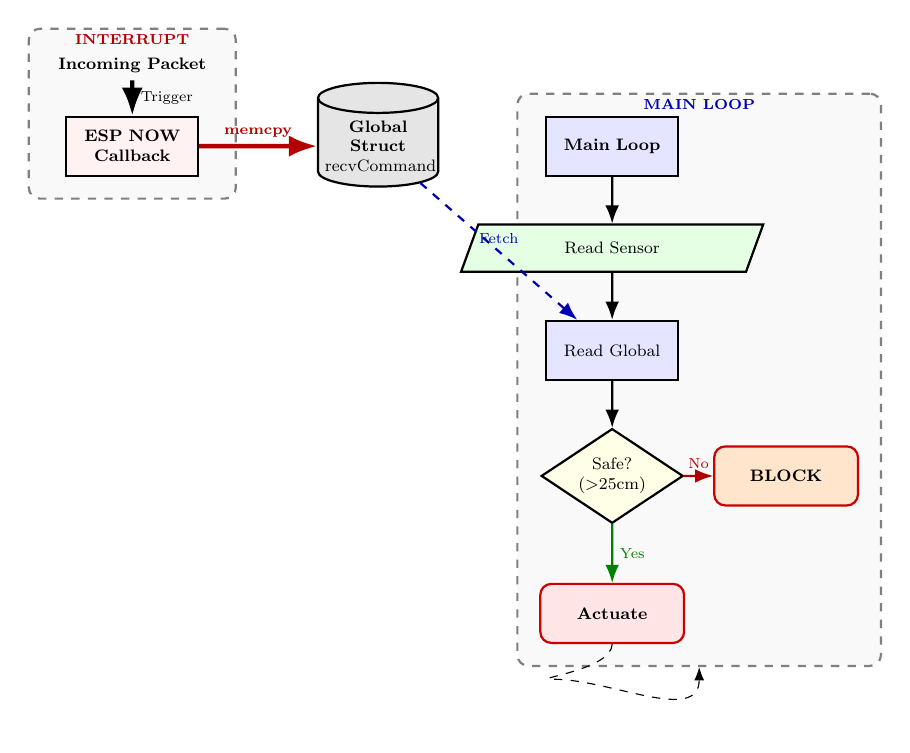
\begin{tikzpicture}[
        scale=0.75, transform shape,
        node distance=1.5cm and 0.8cm, % Reduced distance
        auto,
        >=Latex,
        font=\sffamily\small,
        % Compacted node styles
        block/.style = {rectangle, draw=black, thick, fill=blue!10, text width=2.0cm, align=center, minimum height=1.0cm, font=\footnotesize},
        decision/.style = {diamond, draw=black, thick, fill=yellow!10, text width=1.5cm, align=center, inner sep=0pt, aspect=1.5, font=\footnotesize},
        data/.style = {cylinder, shape border rotate=90, draw=black, thick, fill=gray!20, text width=1.8cm, align=center, minimum height=1.2cm, aspect=0.25, font=\footnotesize},
        sensor/.style = {trapezium, trapezium left angle=70, trapezium right angle=110, draw=black, thick, fill=green!10, text width=2.2cm, align=center, minimum height=0.8cm, font=\footnotesize},
        actuator/.style = {rectangle, draw=red!80!black, thick, fill=red!10, text width=2.2cm, align=center, minimum height=1.0cm, rounded corners, font=\footnotesize},
        line/.style = {draw, thick, ->},
        dashedline/.style = {draw, thick, dashed, ->},
        contextbox/.style = {draw=gray, dashed, thick, rounded corners, fill=gray!5, inner sep=8pt}
    ]

        % --- Left Column: Interrupt Context ---
        \node [block, fill=red!5] (isr) {\textbf{ESP NOW Callback}};
        \node [above=0.6cm of isr, font=\bfseries\footnotesize] (packet) {Incoming Packet};
        \draw [line, ultra thick] (packet) -- node[right, font=\scriptsize] {Trigger} (isr);

        % --- Center: Shared Memory ---
        % Reduced spacing from 3cm to 1.2cm
        \node [data, right=2cm of isr] (sharedMem) {\textbf{Global Struct}\\recvCommand};

        % --- Right Column: Main Loop Context ---
        % Reduced spacing from 3cm to 1.2cm
        \node [block, right=1.8cm of sharedMem] (loopStart) {\textbf{Main Loop}};
        \node [sensor, below=0.8cm of loopStart] (readSensors) {Read Sensor};
        \node [block, below=0.8cm of readSensors] (readGlobal) {Read Global};
        \node [decision, below=0.8cm of readGlobal] (safetyCheck) {Safe?\\($>$25cm)};
        
        % Actuation paths
        \node [actuator, below=1.0cm of safetyCheck] (actuate) {\textbf{Actuate}};
        \node [actuator, right=0.5cm of safetyCheck, fill=orange!20] (blockCmd) {\textbf{BLOCK}};

        % --- Context Boxes (Background layers) ---
        \begin{pgfonlayer}{background}
            \node [contextbox, fit=(packet) (isr), label={[anchor=north,red!70!black,font=\scriptsize]north:\textbf{INTERRUPT}}] (isrContext) {};
            \node [contextbox, fit=(loopStart) (actuate) (blockCmd), label={[anchor=north,blue!70!black,font=\scriptsize]north:\textbf{MAIN LOOP}}] (loopContext) {};
        \end{pgfonlayer}

        % --- Connections ---
        % ISR to Shared Memory
        \draw [line, ultra thick, red!70!black] (isr) -- node[above, font=\scriptsize\bfseries] {memcpy} (sharedMem);

        % Main Loop Flow
        \draw [line] (loopStart) -- (readSensors);
        \draw [line] (readSensors) -- (readGlobal);
        \draw [line] (readGlobal) -- (safetyCheck);

        % Shared Memory to Main Loop
        \draw [dashedline, blue!70!black] (sharedMem) -- node[above, font=\scriptsize] {Fetch} (readGlobal);

        % Safety Decisions
        \draw [line, green!50!black, thick] (safetyCheck) -- node[right, font=\scriptsize] {Yes} (actuate);
        \draw [line, red!70!black, thick] (safetyCheck) -- node[above, font=\scriptsize] {No} (blockCmd);

        % Loopback
        \draw [dashed, ->] (actuate.south) to[out=270,in=180] ++(-1.0,-0.6) to[out=0,in=270] ($(loopContext.south west)!0.5!(loopContext.south east)$);

    \end{tikzpicture}
    \caption{Data flow diagram illustrating the deferred motor actuation design. The high priority ESP NOW callback quickly stores incoming data into shared memory. The lower priority main loop reads the latest sensor data and the stored command, performing safety checks before any physical motor actuation occurs.}
    \label{fig:callback-flow}
\end{figure}

\subsection{Telemetry Transmission}

Telemetry is sent at 2Hz (every 500ms) to avoid flooding the wireless channel. The feedback packet contains battery voltage and ultrasonic distance. The gateway forwards this data to the dashboard over USB serial.

\begin{lstlisting}[language=C++, caption={Telemetry transmission with rate limiting}]
static unsigned long lastTelemetryTime = 0;
static const unsigned long TELEMETRY_INTERVAL = 500;  // 2Hz

void handleConnection(float voltage, int distance) {
    unsigned long now = millis();
    
    // Rate limit to 2Hz
    if (now - lastTelemetryTime >= TELEMETRY_INTERVAL) {
        lastTelemetryTime = now;
        
        sendFeedback.voltage = voltage;
        sendFeedback.distance = distance;
        
        esp_err_t result = esp_now_send(
            gatewayMAC, 
            (uint8_t*)&sendFeedback, 
            sizeof(sendFeedback)
        );
        
        if (result != ESP_OK) {
            Serial.println("Telemetry send failed");
        }
    }
}
\end{lstlisting}

% --------------------------------------------------------
\section{Safety Mechanisms}
\label{sec:safety-mechanisms}

The firmware implements multiple layers of safety to prevent the rover from colliding with obstacles or running away if communication is lost. These mechanisms operate at the firmware level where response time is guaranteed.

\subsection{Heartbeat Failsafe}

If no command packet arrives within 500ms, the rover assumes communication has been lost and stops all motors. This prevents the rover from continuing to execute a stale "forward" command indefinitely. The timeout value was chosen based on the expected packet rate of 20Hz from the joystick.

\begin{lstlisting}[language=C++, caption={Heartbeat check in main control loop}]
const unsigned long SIGNAL_TIMEOUT = 500;  // 500ms

void handleControlLoop() {
    // Check connection heartbeat
    if (!isConnectionAlive(SIGNAL_TIMEOUT)) {
        static bool signalLostPrinted = false;
        if (!signalLostPrinted) {
            Serial.println("SIGNAL LOST - EMERGENCY STOP!");
            signalLostPrinted = true;
        }
        stopMoving();
        return;  // Skip all control logic
    }
    
    // ... rest of control logic
}

bool isConnectionAlive(unsigned long timeoutMs) {
    if (lastPacketTime == 0) return true;  // Allow startup
    return (millis() - lastPacketTime) < timeoutMs;
}
\end{lstlisting}

% FIGURE PLACEHOLDER
\begin{figure}[H]
    \centering
    \includegraphics[width=0.85\textwidth]{figures/software/heartbeat_state_machine.jpg}
    \caption{State machine for heartbeat monitoring showing transitions between connected and stopped states.}
    \label{fig:heartbeat-fsm}
\end{figure}

\subsection{Ultrasonic Obstacle Detection}

The ultrasonic sensor provides distance measurements to the nearest obstacle in the forward direction. The firmware uses this to override forward commands when an obstacle is too close. The implementation uses a state machine rather than the blocking \texttt{pulseIn()} function to avoid freezing the main loop.

\begin{lstlisting}[language=C++, caption={Non blocking ultrasonic state machine}]
enum UltrasonicState {
    US_IDLE,
    US_TRIGGER_HIGH,
    US_WAIT_ECHO_START,
    US_WAIT_ECHO_END
};

static UltrasonicState usState = US_IDLE;
static unsigned long usTriggerTime = 0;
static unsigned long usEchoStart = 0;

bool updateUltrasonicDistance() {
    unsigned long now = micros();
    
    switch (usState) {
    case US_IDLE:
        digitalWrite(TRIG_PIN, HIGH);
        usTriggerTime = now;
        usState = US_TRIGGER_HIGH;
        break;
        
    case US_TRIGGER_HIGH:
        if (now - usTriggerTime >= 10) {  // 10us trigger pulse
            digitalWrite(TRIG_PIN, LOW);
            usState = US_WAIT_ECHO_START;
        }
        break;
        
    case US_WAIT_ECHO_START:
        if (digitalRead(ECHO_PIN) == HIGH) {
            usEchoStart = now;
            usState = US_WAIT_ECHO_END;
        } else if (now - usTriggerTime > 30000) {  // 30ms timeout
            currentDistance = 999;  // No object detected
            usState = US_IDLE;
            return true;
        }
        break;
        
    case US_WAIT_ECHO_END:
        if (digitalRead(ECHO_PIN) == LOW) {
            unsigned long duration = now - usEchoStart;
            currentDistance = (duration * 0.034) / 2;  // Speed of sound
            usState = US_IDLE;
            return true;
        } else if (now - usEchoStart > 30000) {  // Timeout
            currentDistance = 999;
            usState = US_IDLE;
            return true;
        }
        break;
    }
    return false;
}
\end{lstlisting}

% FIGURE PLACEHOLDER
\begin{figure}[H]
    \centering
    \includegraphics[width=\textwidth]{figures/software/ultrasonic_state_machine.jpg}
    \caption{State machine diagram for non blocking ultrasonic distance measurement.}
    \label{fig:ultrasonic-fsm}
\end{figure}

\subsection{Unified Control Loop}

The main control loop integrates all sensor inputs and safety checks before executing motor commands. This unified approach ensures that no command is executed without considering the current safety state.

\begin{lstlisting}[language=C++, caption={Unified control loop with safety integration}]
const int EMERGENCY_STOP_DISTANCE = 25;  // cm

void handleControlLoop() {
    // 0. Check heartbeat (covered above)
    
    // 1. Update distance sensor (non blocking)
    updateUltrasonicDistance();
    
    // 2. Get latest joystick command
    command_struct cmd = getLastCommand();
    
    // 3. Is rover trying to move forward?
    bool tryingToMoveForward = (cmd.y > 2500);
    
    // 4. Safety decision matrix
    if (currentDistance < EMERGENCY_STOP_DISTANCE 
        && tryingToMoveForward) {
        // Block forward movement
        if (!emergencyStopActive) {
            Serial.printf("OBSTACLE at %d cm - BLOCKING!\n", 
                currentDistance);
            stopMoving();
            emergencyStopActive = true;
        }
        
        // But allow backward/turning to escape
        if (cmd.y < 1500 || cmd.x < 1000 || cmd.x > 3000) {
            Serial.println("Escape maneuver allowed");
            executeMotorCommand(cmd.x, cmd.y);
            emergencyStopActive = false;
        }
    } else {
        // Safe to execute command
        emergencyStopActive = false;
        executeMotorCommand(cmd.x, cmd.y);
    }
}
\end{lstlisting}

% FIGURE PLACEHOLDER
\begin{figure}[h!]
    \centering
    \includegraphics[width=\textwidth]{figures/software/control_loop_flowchart.jpg}
    \caption{Flowchart of the unified control loop showing all safety checks and their precedence.}
    \label{fig:control-loop-flow}
\end{figure}

\begin{table}[h!]
    \centering
    \caption{Safety mechanism summary}
    \label{tab:safety-summary}
    \begin{tabular}{llp{5cm}}
        \toprule
        \textbf{Mechanism} & \textbf{Trigger} & \textbf{Action} \\
        \midrule
        Heartbeat failsafe & No packets for 500ms & Stop all motors \\
        Obstacle blocking  & Distance < 25cm + forward command & Block forward, allow escape \\
        Slow zone          & Distance 25-50cm & (Future: reduce speed) \\
        Watchdog timer     & Firmware hang & Hardware reset \\
        \bottomrule
    \end{tabular}
\end{table}

\begin{designbox}[Escape Maneuver Override]
During early testing, we encountered a frustrating scenario: the rover would detect an obstacle at 20cm and freeze completely. The operator could not back up or turn away because all motor commands were blocked by the safety system.

The solution was to make the safety check directional. Forward motion is blocked when an obstacle is close, but \textbf{backward and turning commands are always allowed}. This ensures the rover never gets permanently stuck. The logic checks if the joystick Y value is below 1500 (backward) or if X is at the extremes (<1000 or >3000, meaning a sharp turn). These "escape maneuvers" bypass the emergency stop and allow the operator to retreat safely.

This is a classic example of safety systems needing to be designed with recovery scenarios in mind, not just failure prevention.
\end{designbox}

% --------------------------------------------------------
\subsection{Development Log: Hardware Procurement Saga}
\label{sec:hardware-procurement}

Acquiring the ESP32-S3-CAM module proved to be a significant learning experience about sourcing components for IoT projects. The team went through three iterations of purchasing before obtaining a working unit.

\textbf{Attempt 1: The Wrong Product.}
The first module was ordered from a low cost Chinese seller on Lazada. The listing advertised "ESP32-S3 with OV2640 Camera" at an attractive price. When the package arrived, we discovered the board was an older ESP32 variant without the S3 suffix, and crucially, it had no camera connector at all. The 24-pin FPC socket for the camera was simply absent from the PCB. After contacting the seller and providing photographic evidence, we processed a return.

\textbf{Attempt 2: Dead on Arrival.}
The second attempt was from a more reputable seller with verified reviews. The board arrived and appeared correct: ESP32-S3-WROOM-1 module, 8MB PSRAM, and a proper camera connector. Initial serial output was promising. However, when we ran the camera initialization code, it returned \texttt{ESP\_ERR\_NOT\_FOUND}. We suspected a wiring issue and spent hours debugging before realizing the OV2640 sensor flex cable was connected but the sensor itself had a physical crack across its surface, invisible without magnification. The camera was dead on arrival.

\textbf{Attempt 3: No Pins, No Problem.}
Armed with frustration, we ordered a replacement camera module (just the OV2640, not the entire board) from a third seller. This arrived intact and was verified to work on a test jig. However, when we tried to connect it to the ESP32-S3 board, we discovered the board's GPIO header was unpopulated. The gold pads were present, but no pins were soldered. The product listing had mentioned "with headers" but clearly, this batch was shipped without them.

Rather than waiting for another return and shipment cycle, we contacted a local electronics repair shop near the university. For a small fee, they hand soldered a 2x20 pin header onto the board. The quality was excellent, and the pins aligned perfectly.

\begin{designbox}[IoT Component Sourcing]
\begin{itemize}
    \item Always verify seller reputation and read recent reviews mentioning the specific product variant you need.
    \item "ESP32" is a family with many variants (ESP32, ESP32-S2, ESP32-S3, ESP32-C3). Confirm the exact chip before ordering.
    \item Camera modules are fragile. Inspect the sensor surface under light immediately upon arrival.
    \item Unpopulated headers are common on development boards. Either order from a listing that explicitly shows assembled headers, or budget for local soldering.
    \item Having a local electronics repair contact can save weeks of waiting for returns and replacements.
\end{itemize}
\end{designbox}

% --------------------------------------------------------
\section{Main Loop Structure}
\label{sec:main-loop}

The main loop in \texttt{RescueRobot.ino} coordinates all subsystems at approximately 60Hz. Each iteration performs control processing, video streaming (if UDP mode), and telemetry transmission.

\begin{lstlisting}[language=C++, caption={Main application loop}]
void loop() {
    // 1. Unified Control Loop
    //    (sensor reading + safety checks + motor actuation)
    handleControlLoop();
    
    // 2. Stream video frame (UDP mode only)
    if (USE_UDP_STREAM) {
        streamFrameUDP();
    }
    
    // 3. Transmit telemetry (rate limited to 2Hz internally)
    handleConnection(BATTERY_VOLTAGE, currentDistance);
    
    // 4. Small delay to prevent watchdog triggers
    delay(5);
}
\end{lstlisting}

The 5ms delay at the end of each loop iteration ensures the watchdog timer is not triggered by tight loops. This delay also provides time for the WiFi stack to process incoming packets between iterations.

% FIGURE PLACEHOLDER
\begin{figure}[h!]
    \centering
    \includegraphics[width=\textwidth]{figures/software/loop_timing_diagram.jpg}
    \caption{Timing breakdown of a single main loop iteration showing relative time spent in each subsystem.}
    \label{fig:loop-timing}
\end{figure}

% --------------------------------------------------------
\section{Compilation and Deployment}
\label{sec:compilation}

The firmware is developed using the Arduino framework with ESP32 board support. Compilation requires specific board settings to enable PSRAM and select the correct partition scheme.

\begin{table}[h!]
    \centering
    \caption{Arduino IDE board configuration}
    \label{tab:arduino-config}
    \begin{tabular}{ll}
        \toprule
        \textbf{Setting} & \textbf{Value} \\
        \midrule
        Board           & ESP32S3 Dev Module \\
        PSRAM           & OPI PSRAM \\
        Flash Mode      & QIO 80MHz \\
        Flash Size      & 16MB \\
        Partition Scheme & Huge APP (3MB No OTA / 1MB SPIFFS) \\
        Upload Speed    & 921600 \\
        \bottomrule
    \end{tabular}
\end{table}

The "Huge APP" partition scheme allocates maximum space for application code, which is necessary given the size of the camera driver library. OTA (over the air) updates are disabled in exchange for the larger application partition.

% FIGURE PLACEHOLDER
\begin{figure}[h!]
    \centering
    \includegraphics[width=\textwidth]{figures/software/arduino_board_settings.png}
    \caption{Arduino IDE Tools menu configuration for ESP32-S3 with PSRAM enabled.}
    \label{fig:arduino-settings}
\end{figure}
